\documentclass[hyperref={bookmarks=true}]{beamer}

\usepackage[utf8]{inputenc}  % important for correct displayment of Umlaute (must appear before \title command!)
\usepackage[T1]{fontenc}
\usepackage[english,ngerman]{babel}

\usepackage[german,onelanguage]{algorithm2e}

\usepackage[controls,buttonsize=0.3cm,buttonfg=0.0, buttonbg=1.0]{animate}
\usepackage{tcolorbox}


\usepackage[utf8]{inputenc}
\usepackage[T1]{fontenc} % Note that the encoding and the font should match. If T1 does not look nice, try deleting the line with the fontenc.
\usepackage[english,ngerman]{babel}
%\usepackage{uniinput}  % not a standard package, installation is quite troublesome
\usepackage{lmodern} % vector fonts

\usepackage{geometry}
%\usepackage{fancyhdr}
%\usepackage{blindtext}
%\usepackage{setspace}
\usepackage{cmap} % pro­vides char­ac­ter map ta­bles, which makes PDFs search­able and copy-able (I don't see a difference yet!!!)
\setlength\parindent{0pt} % stop indenting every paragraph by 1cm. It looks awful!

\makeatletter % make @ correct
\@ifpackageloaded{xcolor}
    {\PassOptionsToPackage{table,usenames,dvipsnames}{xcolor}}
    {\usepackage[table,usenames,dvipsnames]{xcolor}}
\makeatother

\usepackage{graphicx} % builds upon the graphics package, providing a key-value interface for optional arguments to the \includegraphics command.
\usepackage{tikz}
\usetikzlibrary{arrows, decorations.markings, calc, datavisualization, datavisualization.formats.functions}
%\usepackage{pgfplots}   %plotting with tex

\makeatletter % make @ correct
% tbtags will put the equation number of a split equation not in the center, but at the top or bottom
\@ifpackageloaded{amsmath}
    {\PassOptionsToPackage{tbtags}{amsmath}}
    {\usepackage[tbtags]{amsmath}}
\makeatother

\usepackage{amsfonts}
\usepackage{amssymb}
%\usepackage{esint}
% bibtex titles are underlined which breaks autor line wrapping!
%http://tex.stackexchange.com/questions/179691/removing-underline-from-journal-title-when-using-hyperref
\usepackage[normalem]{ulem}
\usepackage{bbm}		% sames as above, but won't redefine the better looking ams-mathbb, doesn't contain \mathbbm{0} though
\usepackage{cancel}		% for making a stroke through a calculation
%\usepackage{tensor}
\allowdisplaybreaks     % allow page breaks for longer align-environments
\usepackage{braket} %Bra,Ket,Braket(scaled) vs. bra,ket,braket(smaller)
\usepackage{MnSymbol} %sumint

\usepackage{tabularx}
\newcolumntype{Y}{>{\centering\arraybackslash}X} % centered column of adjustable size i.e. with auto line break
\usepackage{multirow}
\usepackage{multicol}

\usepackage{rotating}	% rotate imported picture
\usepackage{pdflscape}	% rotate site by 90° with \begin{landscape}
%\usepackage{fancyhdr}
\usepackage[binary-units=true]{siunitx}    % SI units paper conform with \SI{3}{\nano\seconds}
                                           % sudo apt-get install texlive-science
\usepackage[labelfont=bf,format=plain]{caption} % enables \captionof for non figure/table environments
%\numberwithin{equation}{chapter}    % equation number contains chapter number
%\numberwithin{figure}{chapter}
%\numberwithin{table}{chapter}

%\usepackage{textcomp}	%for \textdegree
%\usepackage{gensymb}	%for \degree in math mode

\usepackage{url}		%for \url{} command to not get problems with :\\ and other symbols
%\usepackage{breakurl}  % only needed when compiling via dvips/ps2pdf
\usepackage{hyperref}	%for labellinks

\usepackage{attachfile} % insert attachments into pdf O_O
\usepackage{animate}

\usepackage{mdframed}
\usepackage{float}      % enables \begin{figure}[H] to disable floating figure

%%%%%%%%%%%%%%%%%%%%%%%%%%%%%%%%%%%%%%%%%%%%%%%%%%%%%%%%%%%%%%%%%%%%%%%%%%%%%%%%


\renewcommand{\vec}[1]{\overrightarrow{#1}}	%overrightarrow is basically just a bigger vector arrow
\newcommand{\important}[1]{\textcolor{BrickRed}{#1}}
\newcommand{\mat}[1]{\mathbf{#1}}
\newcommand{\mvec}[1]{\underline{#1}} % Vektor in Matrixschreibweise

%\renewcommand{\i}{\text{i}} %normal math i is without point

\newcommand{\de}{\text{d}}
\newcommand{\const}{\text{\small const.}}
\renewcommand{\div}{\text{div}\,}
\renewcommand{\nabla}{\overrightarrow{\bigtriangledown}}
\newcommand{\laplace}{\bigtriangleup}
\newcommand{\grad}{\text{grad}\,}
\newcommand{\rot}{\text{rot}\,}
\newcommand{\dalembert}{\square}
\newcommand{\affects}[1]{\overset{\downarrow}{#1}}
\newcommand{\vecb}[2]{\left(\vec{#1}\right)_{#2}}
\newcommand{\fpart}[2]{\frac{\partial #1}{\partial #2}}
\newcommand{\ftdif}[2]{\frac{\de #1}{\de #2}}
\newcommand{\slfrac}[2]{\left.#1\middle/#2\right.}
\newcommand{\scos}[1]{\text{c}_{#1}\,}
\newcommand{\ssin}[1]{\text{s}_{#1}\,}

%ToDo: Switch between shorter symbols for inverse functions
\newcommand{\invf}[1]{#1^{-1}}				%Inverse function notation

\newcommand{\arsinh}{\text{arsinh}\,}
\newcommand{\arcosh}{\text{arcosh}\,}
\newcommand{\arcoth}{\text{arcoth}\,}
\newcommand{\artanh}{\text{artanh}\,}

\newcommand{\atan}{\text{atan}\,} %short for ArcTan
\newcommand{\asin}{\text{asin}\,}
\newcommand{\acos}{\text{acos}\,}

\newcommand{\ceil}[1] {\left\lceil  #1 \right\rceil}
\newcommand{\floor}[1]{\left\lfloor #1 \right\rfloor}

%Physik
\newcommand{\angstrom}{\overset{\circ}{\text{A}}}
\newcommand{\tesla}{\text{T}}
\newcommand{\unit}[1]{\text{#1}}
%\newcommand{\lagrangian}{\mathcal{L}}
%\newcommand{\lagsecondkind}{\ftdif{}{t}\fpart{\lagrangian}{\dot{q_j}}-\fpart{\lagrangian}{q_j}}


\newcommand{\R}{\mathbb{R}}
\newcommand{\smd}[2]{\sum\limits_{#1}^{#2}} %SuM with Defined boundaries
\newcommand{\ind}[2]{\int\limits_{#1}^{#2}} %INtegral with Defined boundaries

\newcommand{\ex}{\hat{x}}
\newcommand{\ey}{\hat{y}}
\newcommand{\ez}{\hat{z}}

%For use in matrices to denote vectors inside a matrix
\newcommand*{\vertbar}{\vrule}%\rule[1ex]{0.5pt}{2.5ex}}
\newcommand*{\horzbar}{\rule[.5ex]{2.0ex}{0.5pt}}	%[Vertical-Shift]{Length}{Thickness}

%Unicodes
\DeclareUnicodeCharacter{2208}{\ensuremath{\in}}
\DeclareUnicodeCharacter{2115}{\ensuremath{\mathbb N}}
\DeclareUnicodeCharacter{2124}{\ensuremath{\mathbb Z}}
\DeclareUnicodeCharacter{2192}{\ensuremath{\rightarrow}}

%QT
\newcommand{\mean}[1]{\langle #1 \rangle}
\newcommand{\esk}[1]{\textcolor{BrickRed}{#1}}	%Einsteinsche Summenkonvention Marker

%Math
\newcommand{\HR}{\mathcal{H}} %Hilbertraum
\newcommand{\solvefor}[1]{\textcolor{Blue}{#1}}



%%%%%%%%%%%%%%%%%%%%%%%%%%%%%%%%%%%%%%%%%%%%%%%%%%%%%%%%%%%%%%%%%%%%%%%%%%%%%%%%


\definecolor{mygreen}{rgb}{0,0.6,0}
\definecolor{mygray}{rgb}{0.5,0.5,0.5}
\definecolor{mymauve}{rgb}{0.58,0,0.82}

\usepackage{listings}   % source code listings
\usepackage{textcomp}   % for upquotes inside lstlisting

\usepackage{courier}    % for lstlisting

\lstset{ %
  backgroundcolor=\color{white},   % choose the background color; you must add \usepackage{color} or \usepackage{xcolor}
  basicstyle=\footnotesize\ttfamily, % the size of the fonts that are used for the code
  breakatwhitespace=false,         % sets if automatic breaks should only happen at whitespace
  breaklines=true,                 % sets automatic line breaking
  captionpos=b,                    % sets the caption-position to bottom
  commentstyle=\color{mygreen},    % comment style
%  deletekeywords={...},            % if you want to delete keywords from the given language
  escapeinside={\%*}{*)},          % if you want to add LaTeX within your code
  extendedchars=false,              % lets you use non-ASCII characters; for 8-bits encodings only, does not work with UTF-8
  %frame=single,                    % adds a frame around the code
  keepspaces=true,                 % keeps spaces in text, useful for keeping indentation of code (possibly needs columns=flexible)
  keywordstyle=\color{blue},       % keyword style
  morekeywords={*,...},            % if you want to add more keywords to the set
  numbers=left,                    % where to put the line-numbers; possible values are (none, left, right)
  numbersep=5pt,                   % how far the line-numbers are from the code
  numberstyle=\tiny\color{mygray}, % the style that is used for the line-numbers
  rulecolor=\color{black},         % if not set, the frame-color may be changed on line-breaks within not-black text (e.g. comments (green here))
  showspaces=false,                % show spaces everywhere adding particular underscores; it overrides 'showstringspaces'
  showstringspaces=false,          % underline spaces within strings only
  showtabs=false,                  % show tabs within strings adding particular underscores
  stepnumber=1,                    % the step between two line-numbers. If it's 1, each line will be numbered
  stringstyle=\color{mymauve},     % string literal style
  tabsize=2,                       % sets default tabsize to 2 spaces
  title=\lstname,                  % show the filename of files included with \lstinputlisting; also try caption instead of title
  xleftmargin=.25in,               % indent listings by default
  upquote=true                     % single quotes '' appear straight instead of as backticks. Needs textcomp
}
\lstdefinelanguage{diff}{
  morecomment=[f][\color{blue}]{@@},     % group identifier
  morecomment=[f][\color{red}]-,         % deleted lines
  morecomment=[f][\color{green}]+,       % added lines
  morecomment=[f][\color{magenta}]{---}, % Diff header lines (must appear after +,-)
  morecomment=[f][\color{magenta}]{+++},
}

% http://tex.stackexchange.com/questions/2644/how-to-prevent-a-page-break-before-an-itemize-list
\makeatletter
\newcommand{\nolisttopbreak}{\vspace{\topsep}\nobreak\@afterheading}
\makeatother

 


\newcommand{\setmathmargin}[1]{
	\setlength{\abovedisplayskip}{#1}
	\setlength{\abovedisplayshortskip}{\abovedisplayskip}
	\setlength{\belowdisplayskip}{\abovedisplayskip}
	\setlength{\belowdisplayshortskip}{\abovedisplayskip}
}

%    \makeatletter
%    \newenvironment{myalign*}{%
%    \setlength{\mathindent}{0pt}%
%    \setlength{\abovedisplayskip}{-\baselineskip}%
%    \setlength{\abovedisplayshortskip}{\abovedisplayskip}%
%    \start@align\@ne\st@rredtrue\m@ne
%    }%
%    {\endalign}
%    \makeatother

%=========== OPTIONS =============

%colorname!integer in percent

\mode<presentation>
{
	%\usetheme{Dresden}
	
	\setbeamercovered{transparent=10}  % transparency of not shown yet items
	\beamertemplatenavigationsymbolsempty
	
	%\useoutertheme[footline=empty,subsection=false]{miniframes}
	\useoutertheme[subsection=false]{miniframes}
	\usecolortheme{whale}
	
}

\makeatletter
\setbeamertemplate{footline}
{
    \begin{beamercolorbox}[colsep=1.5pt]{upper separation line foot}
    \end{beamercolorbox}
%    %%%%%%%% horizontal line containign authors and institute %%%%%%%%
%    \begin{beamercolorbox}[
%    	ht=2.5ex,
%    	dp=1.125ex,
%	    leftskip=.3cm,
%	    rightskip=.3cm plus1fil
%	]{author in head/foot}
%        \leavevmode{\usebeamerfont{author in head/foot}\insertshortauthor}
%	    \hfill
%        {
%       		\usebeamerfont{institute in head/foot}
%        	\usebeamercolor[fg]{institute in head/foot}
%        	\insertshortinstitute
%        }
%    \end{beamercolorbox}
    %%%%%%%% Horizontal bar containing title and frame numbers %%%%%%%%
    \begin{beamercolorbox}[
    	ht=2.5ex,
    	dp=1.125ex,
      	leftskip=.3cm,
      	rightskip=.3cm plus1fil
    ]{title in head/foot}%
        {\usebeamerfont{title in head/foot}\insertshorttitle}
        \hfill
        {
        	\usebeamerfont{frame number}
        	\usebeamercolor[fg]{frame number}
        	\insertframenumber~/~\inserttotalframenumber
        }
    \end{beamercolorbox}%
    \begin{beamercolorbox}[colsep=1.5pt]{lower separation line foot}
    \end{beamercolorbox}
}
\makeatother

%	\pgfdeclareimage[height=0.5cm]{tud-logo}{logo_weiss.pdf}
%	\logo{\pgfuseimage{tud-logo}}

% Delete this, if you do not want the table of contents to pop up at
% the beginning of each subsection:
%\AtBeginSection[]{
%  \begin{frame}<beamer>{Übersicht}
%    \tableofcontents[currentsection,currentsubsection]
%  \end{frame}
%}

% If you wish to uncover everything in a step-wise fashion, uncomment
% the following command: 
%\beamerdefaultoverlayspecification{<+->}

\title{Master ''Computational Science and Engineering''\\
       Belegarbeit: Verteilte GPGPU-Berechnungen mit Spark}
\author {
	Maximilian Knespel
	\newline	\newline
	Betreuer: \and Dipl.-Inf. Nico Hoffmann
}
\date{}
%\date{7. Juli 2016}


\begin{document}

\begin{frame}
	\titlepage
\end{frame}

%\begin{frame}
%	\frametitle{Outline}
%	\setcounter{tocdepth}{1}
%	\tableofcontents
%\end{frame}


%%%%%%%%%%%%%%%%%%%%%%%%%%%%%%%%%%%%%%%%%%%%%%%%%%%%%%%%%%%%%%%%%%%%%%%%%%%%%%%%
\section{Einführung}
%%%%%%%%%%%%%%%%%%%%%%%%%%%%%%%%%%%%%%%%%%%%%%%%%%%%%%%%%%%%%%%%%%%%%%%%%%%%%%%%


\begin{frame}
    \frametitle{GPU-Beschleuniger zum Hochleistungsrechnen}
    % Bild K20x und AmdOpteron ? damit man sofort sieht, um was es auf der Folie geht?
    %  - https://commons.wikimedia.org/wiki/File:AMD_Opteron_2212_IMGP1795.jpg
    %  - http://images.nvidia.com/content/tesla/images/tesla-3-quater.png
    %
    % sagen:
    %   - Mittlerweile ist GPU an vielen Stellen schon Mainstream im Cluster-
    %     Computing geworden. Beispielhafter Beweis: die aktuelle Top 3 Titan XK7:
    %         18 688 AMD Opteron 6274 (16 Kerne)
    %         18 688 Nvidia Tesla K20X (90% der Rechenlast)
    %       https://www.olcf.ornl.gov/titan/
    %     und viele andere haben auch schon oder wollen aufrüsten
    %     Top 8 will dieses Jahr mit 4500 Pascal GPUs (16nm HBM2) aufrüsten
    %       http://nvidianews.nvidia.com/news/nvidia-pascal-gpus-to-double-speed-of-europe-s-fastest-supercomputer
    %     https://www.top500.org/lists/2016/06/
    %     http://on-demand.gputechconf.com/supercomputing/2012/presentation/SB005-Bland-Titan-Oak-Ridge-National-Labs.pdf
    %
    \begin{columns}\begin{column}{0.5\linewidth}
        \centerline{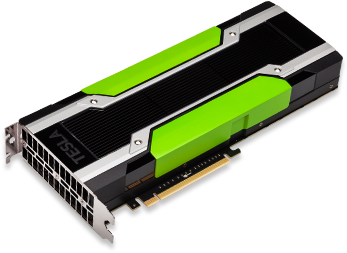
\includegraphics[height=0.15\textheight]{tesla-3-quater.png}}
        %\textcolor{gray}{\scriptsize{NVIDIA}}
    \end{column}\begin{column}{0.5\linewidth}
        \centerline{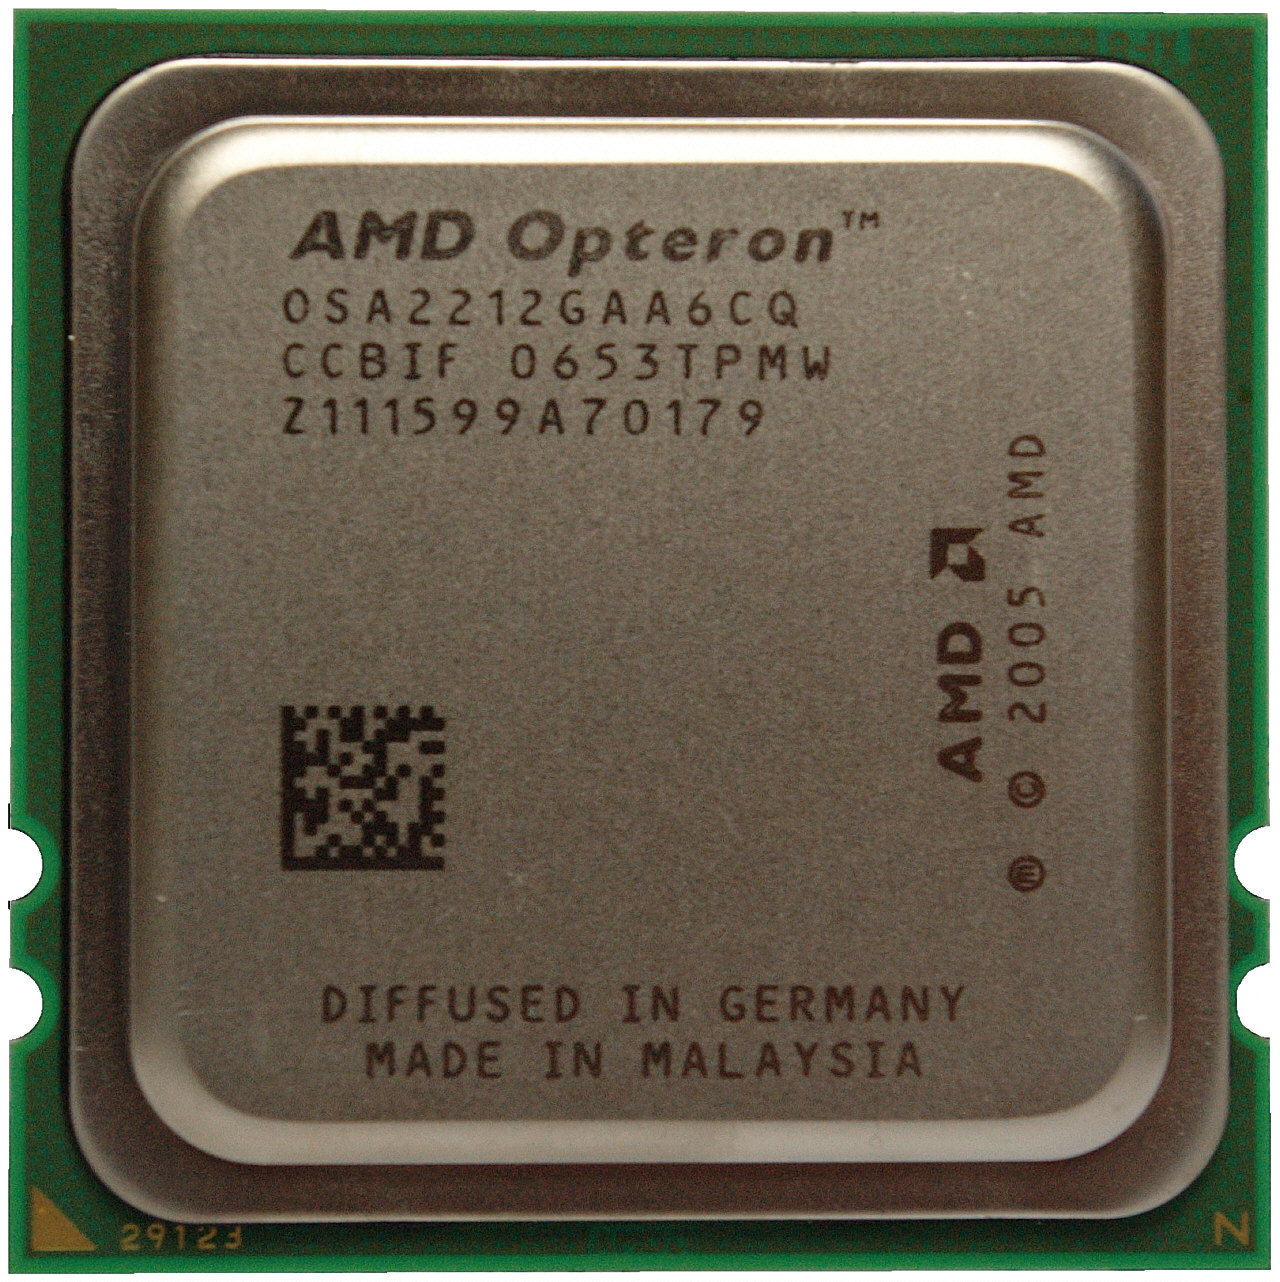
\includegraphics[height=0.15\textheight]{AMD_Opteron_2212_IMGP1795.jpg}}
        %\textcolor{gray}{\scriptsize{Rainer Knäpper, Free Art License (\url{artlibre.org/licence/lal/en/})}}
    \end{column}\end{columns}
    Platz 3 Titan XK7 in der Top 500 (Juni 2016):
    \begin{itemize}
        \item 18 688 AMD Opteron 6274 (16 Kerne) zu je 140\,TFLOPS(DP)
        \item 18 688 Nvidia Tesla K20X zu je 1.3\,TFLOPS(DP)  % (90% der Rechenlast)
    \end{itemize}
    % Ist eigtl. eher general knowledge, aber kann ja nicht schaden, als kleiner Einstieg, außer wenn ich dadurch ein Halbwissen zur Schau stelle.
    General Purpose Graphical Processing Units (GPGPU) im Vergleich zu Prozessoren:
    \begin{itemize}
        %\item[+] Kosteneffektiv in Anschaffung
        \item[+] bessere Leistungsaufnahme pro GFlops
        \item[–] nur für bestimmte Anwendungen geeignet
            % sagen:
            %  - niedrig Latenz, streaming (in Bezug auf Speicehrzugriffe)
            %    (wenige random access)
            %  - eher für compute-bound (auf CPU) Probleme geeignet
        \item[+] hohe Speicherbandbreiten
        \item[–] hohe Speicherlatenzen
        \item[+] massiv parallel %(3840 CUDA cores gegen 24 cores Xeon E7-8890-v4 (AVX2)
            % (Broadwell 14nm) http://ark.intel.com/products/91317/Intel-Xeon-Processor-E5-2699-v4-55M-Cache-2_20-GHz
            % http://ark.intel.com/de/products/93790/Intel-Xeon-Processor-E7-8890-v4-60M-Cache-2_20-GHz
            % http://www.cpu-world.com/info/id_model/Intel-server-conventions.html
            %   E7: Mission-critical
            %   v4: Broadwell
            % Broadwell AVX2 (256-Bits => 8 floats) (FMA*2) => entspricht also 24*8*2 CUDA-Cores = 384 -> Faktor 10 langsamer (meist nochmal Faktor 2 wegen kleiner Taktfrequenz von GPUs). Faktor 10,5 stimmt gut mit empirischen Messungen überein.
        \item[–] \textbf{zusätzliche Komplexität beim Programmieren}
    \end{itemize}
    % sagen:
    %  - Ziel dieser Belegarbeit ist es den letzten Punkt zu tilgen, indem man Berechnungen auf GPUs in das Spark-Framework einbringt (in nächsten Folien dann klar machen, dass die high-level Befehle in Spark sehr praktisch sind, um die GPU-Programmierung zu verstecken (map reduce abstraktion))
\end{frame}



%%%%%%%%%%%%%%%%%%%%%%%%%%%%%%%%%%%%%%%%%%%%%%%%%%%%%%%%%%%%%%%%%%%%%%%%%%%%%%%%
\section{Spark}
%%%%%%%%%%%%%%%%%%%%%%%%%%%%%%%%%%%%%%%%%%%%%%%%%%%%%%%%%%%%%%%%%%%%%%%%%%%%%%%%

% Following:
%  - https://www.toptal.com/spark/introduction-to-apache-spark
%  - "Learning Spark" book

\begin{frame}
    \frametitle{MapReduce Programmiermodell}
    % nicht sicher in welchen Zitationsstil ich das hier machen soll, oder einfach nur freihand?
    ''MapReduce: Simplified Data Processing on Large Clusters'' (2004) von Jeffrey Dean und Sanjay Ghemawat (Google Inc.)
    %@article{
    %    author     = {Dean, Jeffrey and Ghemawat, Sanjay},
    %    title      = {MapReduce: Simplified Data Processing on Large Clusters},
    %    journal    = {Commun. ACM},
    %    issue_date = {January 2008},
    %    volume     = {51},
    %    number     = {1},
    %    month      = jan,
    %    year       = {2008},
    %    issn       = {0001-0782},
    %    pages      = {107--113},
    %    numpages   = {7},
    %    url        = {http://doi.acm.org/10.1145/1327452.1327492},
    %    doi        = {10.1145/1327452.1327492},
    %    acmid      = {1327492},
    %    publisher  = {ACM},
    %    address    = {New York, NY, USA},
    %}
    \begin{itemize}
        \item Für Cluster aus tausenden von kommerziellen PCs entwickelt % (inexpensive HDDs) reliability on top of unreliable hardware
        \item MapReduce bezeichnet ein Programmiermodell und die dazugehörige Implementation
        \item Schlüssel/Wert-Paare auf die eine Abbildung und nachfolgend eine Reduktion aller Werte eines Schlüssels ausgeführt wird
              \begin{tabular}{lll}
                  Map     & : $(k,v)$ &
                              $\mapsto \left[(l_1,x_1), \ldots, (l_{r_k},x_{r_k}) \right]$ \\
                  %Shuffle & : $\left[(l_1,x_1), \ldots, (l_{r_k},x_{r_k}) \right]$ &
                  %            $\mapsto (l,\left[ y_1, \ldots, y_{s_l} \right])$ \\
                  Reduce  & : $(l,\left[ y_1, \ldots, y_{s_l} \right])$ &
                              $\mapsto \left[ w_1, \ldots, w_{m_l} \right] $
              \end{tabular}
        % viele aufgaben lassen sich in dieses map+reduce schema pressen (turing vollständig?... ka)
        \item Programme in diesem funktionalen Stil werten automatisch von MapReduce parallelisiert
        % runtime macht dabei automatisch eine partitionierung und kümmert sich um lastbalancierung, Kommunikation der Input und Output-Daten, Fehlertoleranzm ...
        % von Google aus der Not heraus entworfen riesige Daten z.B. zusammenzufassen und mit Graphenalgoritmen Webseiten zu bewerten
        % inspiriert von funktionalen Sprachen wie Lisp (map, reduce)
    \end{itemize}
\end{frame}


\begin{frame}
    \frametitle{Spark Übersicht}
    % Sagen:
    %  - 2009 als Forschungsprojekt am UC Berkely Lab angefangen
    %  - 2013 Transfer zur Apache Software Foundation
    %  - GraySort Gewinner 5.11.2014: Apache Spark von Reynold Xin (Databricks Inc.)
    %     => 3x schneller bei 1/10 Knoten und 1/5 Datendurchsatz als alter Hadoop MapReduce-Gewinner
    %     => ab da wsl. richtig an Fahrt gewonnen
    %\begin{itemize}
    %    \item Nachfolger zu Hadoop MapReduce
    %    \item geschrieben in Scala
    %\end{itemize}
    % (Hadoop: Core MapReduce + verteiltes Dateisystem(HDFS,NFS,...))
    Nachfolger von Hadoop MapReduce. Vorteile:
    \begin{itemize}
        \item[+] Abarbeitung im Arbeitsspeicher möglich % , was Hadoop nicht anbot
        \item[+] iterative Algorithmen schneller als Hadoop % wegen cache/persist-Funktionen
            % auch auf der Festplatte schneller als Hadoop MapReduce! % WARUM?!
            % http://stackoverflow.com/questions/26870537/spark-what-is-the-difference-between-cache-and-persist
            % cache only memory <-> persist can specify, e.g. disk
        \item[+] mehr und komplexere Methoden % Komplexbefehle zur Verfügung
        \item[+] interaktive Konsole % zum schnellen Prototyping
        % vereinfachtere Programmierung gegenüber simplen MapReduce
        %   -> siehe nächste Folie
        \item[+] Unterstützung für: Scala, Java, Python, \ldots
        \item[+] lokales Dateisystem, HDFS, AmazonS3, \ldots nutzbar % (Hadoop erzwingt HDFS), HDFS u.a. auch in Spark möglich
    \end{itemize}
\end{frame}

\begin{frame}[fragile]
    % Data sharing is slow in MapReduce due to replication, serialization, and disk IO. Most of the Hadoop applications, they spend more than 90% of the time doing HDFS read-write operations. -> http://www.tutorialspoint.com/spark_sql/spark_sql_quick_guide.htm
    \frametitle{Resilient Distributed Datasets (RDDs)}
    \begin{itemize}
        \item zu bearbeitende Daten liegen in RDD-Objekten
        % sagen:
        %  - sind eine Abstraktion von Daten, können erstellt werden z.B. durch Einlesen von Dateien z.B. in HDFS oder durch parallelize auf eine bestehende "collection"(?)
        \item Resilience: opake Neuberechnung der Teildaten bei Absturz eines Knotens möglich
        \item Methoden zur Verarbeitung der Daten
              \begin{tcolorbox}[boxsep=0pt]
                \begin{lstlisting}[language=scala,numbers=none,xleftmargin=0pt,escapeinside={(*}{*)}]
def filter(f: (T) (*$\Rightarrow$*) Boolean): RDD[T]
\end{lstlisting}\vspace{-1.5\baselineskip}
              Return a new RDD containing only the elements that satisfy a predicate.
              \end{tcolorbox}
              %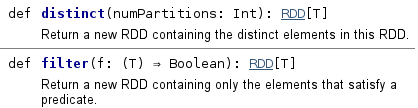
\includegraphics[width=0.9\linewidth]{rdd-disting-filter.png}\\
              %\textcolor{gray}{\scriptsize{\url{
              %   https://spark.apache.org/docs/0.8.1/api/core/org/apache/spark/rdd/RDD.html
              %}}}
              % Bild soll für Programmierer zeigen, dass es wirklich nicht viel mehr als eine Klassenabstraktion ist, indem es Methoden dieser Klasse zeigt
        %\item distributed:
        \item ist aufgeteilt in Partitionen, welche auf verschiedenen Knoten berechnet werden können % mehr partionen -> bessere lastbalancierung möglich
    \end{itemize}
    % https://spark.apache.org/docs/1.5.2/api/scala/index.html#org.apache.spark.SparkContext
\end{frame}


\begin{frame}
    \frametitle{Spark Funktionsweise}
    \centerline{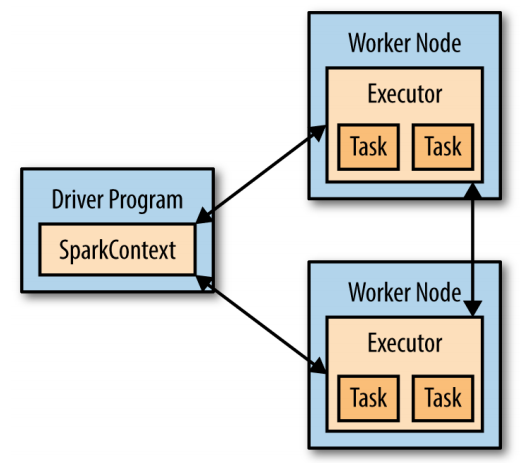
\includegraphics[width=0.7\linewidth]{spark-components-execution.png}}
    % spark opak gegenüber cluster manager, so lange man programme starten kann -> siehe Kapitel implementation
    % driver programm muss von allen worker erreichbar sein
    % spark hat auch job scheduling und übernimmt damit einige Funktionen von slurm / pbs (not user)
    % hat nettes webinterface mit logs und zustand ...
\end{frame}


\begin{frame}
    \frametitle{Spark Anwendungen}
    % - datenanalyse, -visualisierung, prognosemodelle (z.B. "you also might like these products ...")
    \centerline{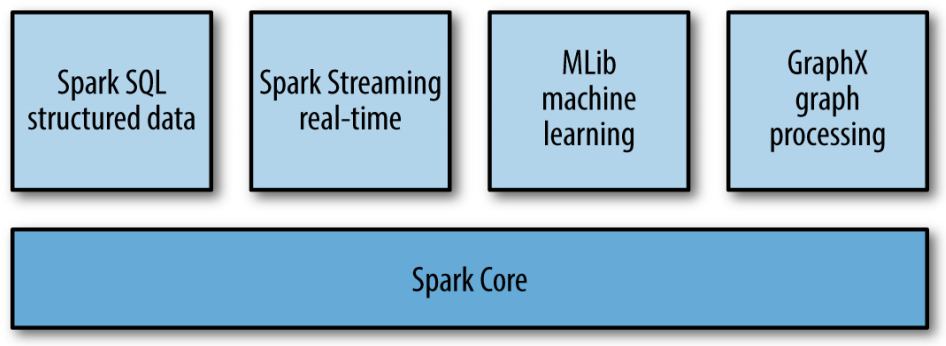
\includegraphics[width=0.8\linewidth]{spark-libraries.png}}
    % sagen:
    %   - Spark SQL:
    %       - allow access to RDDs using SQL queries über einen SQL Kontext:
    %           val schemaString = "name age"
    %           ...
    %           val rowRDD = people.map(_.split(",")).map(p => Row(p(0), p(1).trim))
    %           val peopleDataFrame = sqlContext.createDataFrame(rowRDD, schema)
    %           val results = sqlContext.sql("SELECT name FROM people")
    %         SchemaRDD
    %       http://spark.apache.org/docs/latest/sql-programming-guide.html#programmatically-specifying-the-schema
    %
    %   - Spark Streaming: Echtzeitdatenanalyse (z.B. Themen / häufigste Wörter in den letzten 10k Tweets). oder Kombination mit MLib möglich (Streaming Linear Regression)
    %     Data fitting während daten gestreamt werden (ich stelle mir z.B. least square fitting von einem physikalischen Experiment vor, z.B. v(t) fitting auf v(t)=v0+g*t fitting, um die Fallbeschleunigung g zu bestimmen, während gemessen wird. (Minimalbeispiel, denkbarer wäre wohl irgendetwas am LHC, mit ihren Terabyte an Daten pro Sekunde) -> Vorteil, dass die Daten nicht gespeichert werden müssen, was vlt. gar nicht möglich wäre:
    %           http://spark.apache.org/docs/latest/mllib-linear-methods.html#streaming-linear-regression
    %
    %   - MlLib: statistiken (mittelwert, standardabweichung, ...), korrelaton, (lineare) regression, k-means, stochastic(online) gradient descent ...
    %       http://spark.apache.org/mllib/
    %       http://spark.apache.org/docs/latest/ml-guide.html
    %       http://spark.apache.org/docs/latest/mllib-optimization.html
    %     Primitiven für Machinenlernen, aber keine highlevel abstraktion wie z.B. Keras, wo das Training in einer Zeile geht:
    %            model.fit( X_train, y_train,
    %                       nb_epoch=1000, batch_size=100,
    %                       verbose=1, validation_split=0.2,
    %                       callbacks=[EarlyStopping( monitor='val_loss',
    %                                                 patience=25, mode='min'),
    %                       WeightLogger()] )
    %               www.thoughtly.co/blog/deep-learning-lesson-3/
    %       (verstehe ich das so richtig ???)
    %       http://www.kdnuggets.com/2015/12/spark-deep-learning-training-with-sparknet.html
    %
    %   - GraphX
    %       Graphdatentyp + Algorithmen drauf wie
    %           PageRank: Berechnung der Relevanz / Popularität aller Knoten in einem Graphen aus den Wertungen ihrer jeweiligen Kanten
    %           subgraph ...
    %       http://spark.apache.org/docs/latest/graphx-programming-guide.html#graph_algorithms
\end{frame}


\begin{frame}
    \frametitle{Spark auf Github}
    \centerline{\url{github.com/apache/spark.git master}}
    % sagen:
    %   - anhaltende >aktive< Entwicklung (nicht wie Rootbeer ...)
    %   - 2012 nur 20k Code, nun 1 Millionen Zeilen -> betonen, um zu zeigen, dass es ein komplexes Projekt ist, für dass ein Mitwirken (GPU Plugin) möglicherweise den Rahmen einer Belegarbeit sprengt ... :)"
    %   - über tausend (1203 an 2016-07-06) Beitragende / Programmierer (210 in den letzten 30 Tagen)
    %   - 33 417 commits
    \centerline{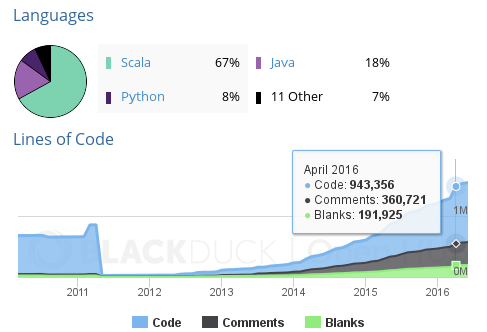
\includegraphics[width=0.9\linewidth]{spark-openhub.png}}
    \centerline{\textcolor{gray}{\scriptsize{\url{
        https://www.openhub.net/p/apache-spark
    }}}}
    % git://github.com/apache/spark.git master
\end{frame}


\begin{frame}
    \frametitle{Monte-Carlo-Integration}
    % sagen:
    %   - kurze Monte-Carlo-Simulation erklären
    %   - mag sinnlos erscheinen für das Beispiel, hat aber Anwendung für komplexere Probleme
    %   - und für höherdimensionale Integration, da der Fehler auf das Integral trotz hoher Dimension mit 1/sqrt(N) sinkt
    %       anstatt in 1D O(dx) =O(1/N), 2D: O(dx*dx * N) (*N wegen Anzahl an Integrationsminifläche, die an dem Rand liegen, welcher 1D ist, d.h. der Umfang (Fraktale mal ausgenommen ...)) => O(1/N**2*N) = O(1/N) man bemerke, dass N die Anzahl an Subintervallen in EINER Dimension, sei also M=O(N^2) die Anzahl an Subvolumen => 2D: O( 1/sqrt(M) ) (für 2D Monte-Carlo-Pi also gleich schnell wie simplestes Integrationsverfahren) -> aber für nD -> O( 1 / n-th root M ) viel langsamer als O( 1 / sqrt(M) ) !
    %       nicht sicher ob Mathematik erwähnen, finde den Fakt ziemlich cool, aber wohl off-topic -> falls ich nicht auf 30min komme
    \begin{columns}\begin{column}{0.35\linewidth}
        \centerline{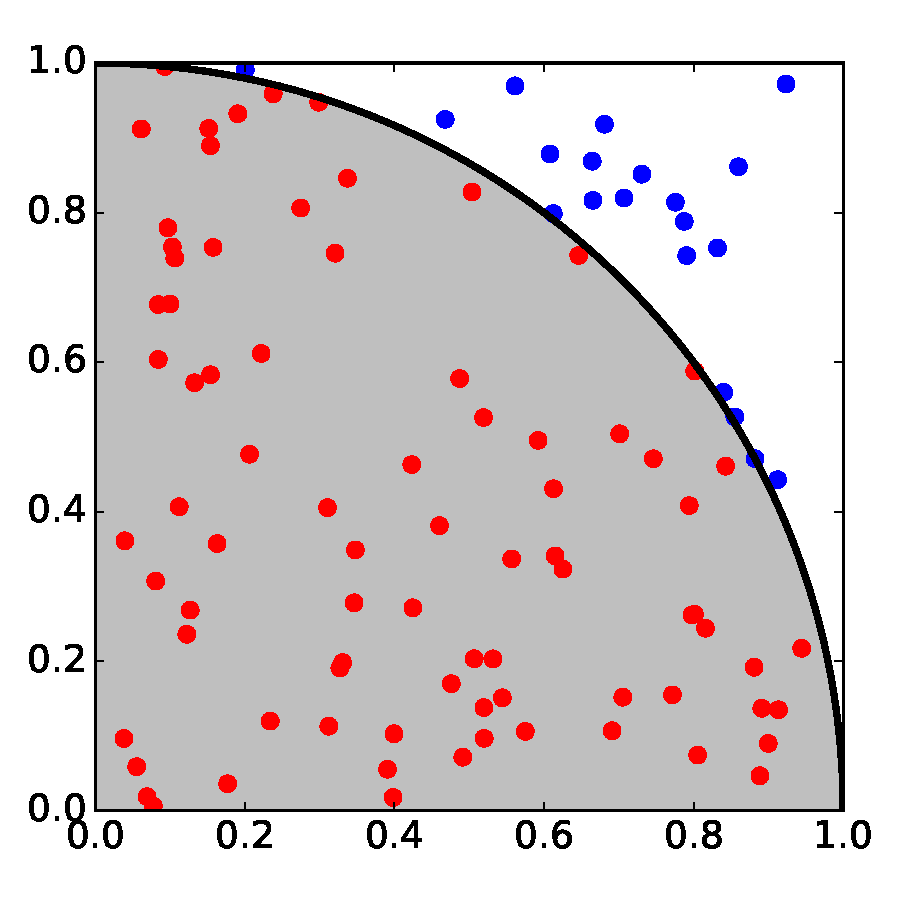
\includegraphics[width=1.1\linewidth]{monte-carlo-pi-quarter-sphere.pdf}}
        % eigener plot:
        %   #!/usr/bin/python
        %
        %   from matplotlib.pyplot import *
        %   from numpy import *
        %
        %   fig = figure( figsize=(6,6) )
        %   ax = fig.add_subplot( 111,
        %       aspect='equal',
        %
        %       xlim=[0,1],
        %       ylim=[0,1]
        %   )
        %   x = random.rand(100)
        %   y = random.rand(100)
        %   inside = x*x + y*y < 1.0
        %   ax.plot( x[inside], y[inside], 'r.', markersize=16 )
        %   ax.plot( x[logical_not( inside )], y[logical_not( inside )], 'b.', markersize=16 )
        %   x = linspace(0,1,1000)
        %   ax.plot(x, sqrt( 1 - x*x ), 'k-', linewidth=2 )
        %
        %   for tick in ax.xaxis.get_major_ticks():
        %         tick.label.set_fontsize(18)
        %   for tick in ax.yaxis.get_major_ticks():
        %         tick.label.set_fontsize(18)
        %   tight_layout()
        %   fig.savefig( "monte-carlo-pi-quarter-sphere.pdf" )
        %
        %   show()
    \end{column}\begin{column}{0.65\linewidth}
        \centerline{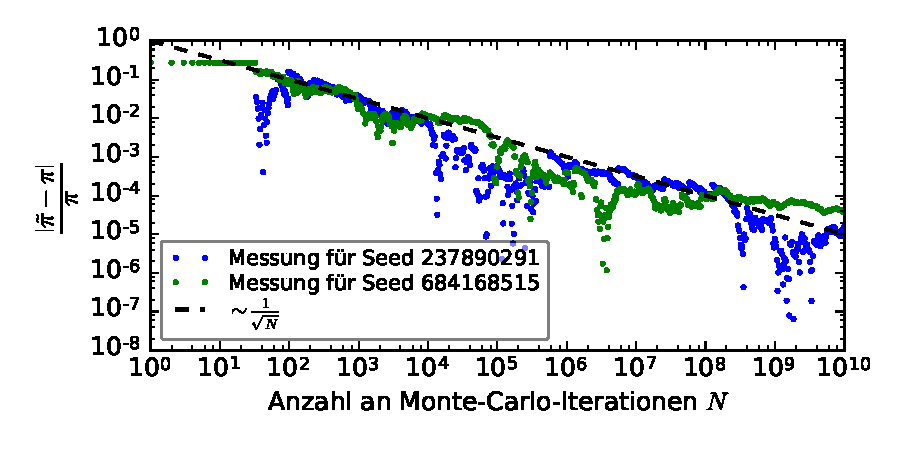
\includegraphics[width=1.1\linewidth]{monte-carlo-pi-error-scaling.pdf}}
        % eigener Plot: python plot.py -e ./raw-logs/cpp-pin-237890291.log 'Messung für Seed 237890291' ./raw-logs/cpp-pin-684168515.log 'Messung für Seed 684168515'
    \end{column}\end{columns}
\end{frame}

\begin{frame}[fragile]
    \frametitle{Implementation Monte-Carlo-Pi-Berechnung}
    \begin{lstlisting}[language=scala]
def calcQuarterPi (
    nIterations : Long,
    rSeed       : Long
) : Double = {
  var seed      = rSeed
  var nHits     = 0L
  val randMax   = 0x7FFFFFFF
  val randMagic = 950706376L
  var i = 0; while ( i < nIterations ) {
    seed  = ( ( randMagic * seed ) % randMax ).toInt
    val x = seed
    seed  = ( ( randMagic * seed ) % randMax ).toInt
    val y = seed
    if ( 1L*x*x + 1L*y*y < 1L*randMax*randMax )
        nHits += 1
    i += 1
  }
  return nHits.toDouble / nIterations
}
\end{lstlisting}
% double can hold up to integer 2**53 exactly
\end{frame}

% http://tex.stackexchange.com/questions/130109/cant-insert-code-in-my-beamer-slide
\begin{frame}[fragile]
    % Beispiel für wie "einfach" die Parallelisierung mit Spark ist, wobei
    % die calcQuarterPi-Funktion erst später erklärt/gezeigt wird
    \frametitle{Spark Monte-Carlo-Pi-Beispiel}
    \begin{lstlisting}[language=bash]
"$SPARK_ROOT"/bin/spark-shell --master local[*]
\end{lstlisting}\vspace{-1.5\baselineskip}
    %\lstset{xleftmargin=0, linewidth=1.05\linewidth}
    \begin{lstlisting}[language=scala]
val sparkConf   = new SparkConf().setAppName("Pi")
var sc          = new SparkContext( sparkConf )
val seed0       = 87541459l
val nPartitions = 100
val nIterations = 1e8.toLong
val quarterPis  = sc.parallelize(1 to nPartitions).
  map( iRank => ( {
    val seed  = ( seed0 + ( iRank.toDouble / nPartitions * Integer.MAX_VALUE ).toLong ) % Integer.MAX_VALUE
    calcQuarterPi( nIterations, seed ) ).cache
quarterPis.take(4).foreach( x => print( x + " " ) )
println( "pi = " + 4*quarterPis.reduce(_+_)/nPartitions )
\end{lstlisting}\vspace{-1.5\baselineskip}
    % Scala Bug / Feature, the normal for loop: (erwähnen, falls sich einer wundert, warum ich while statt for nehme ... -.-
    %    for ( i <- 0 to 2147483647 ) x+=1
    % will fail with:
    % java.lang.IllegalArgumentException: 0 to 2147483647 by 1: seqs cannot contain more than Int.MaxValue elements.
    % http://stackoverflow.com/questions/9888706/why-is-the-scala-for-loop-and-internals-numericrange-restricted-to-int-size-an
    Programmausgabe:
    \begin{lstlisting}
0.7852178 0.7852558 0.7855507 0.78554
pi = 3.1415955324
\end{lstlisting}\vspace{-1.5\baselineskip}
\end{frame}



%%%%%%%%%%%%%%%%%%%%%%%%%%%%%%%%%%%%%%%%%%%%%%%%%%%%%%%%%%%%%%%%%%%%%%%%%%%%%%%%
\section{Rootbeer}
%%%%%%%%%%%%%%%%%%%%%%%%%%%%%%%%%%%%%%%%%%%%%%%%%%%%%%%%%%%%%%%%%%%%%%%%%%%%%%%%
%%%%NH: hier eine Einführung Rootbeer (Paper referenzieren + kurz erklären -> insb. mit Übersetzung in 3 adress code etc. ..)


\begin{frame}
    \frametitle{GPU-Programmierung mit Java/Scala}
    \begin{itemize}
        \item OpenCL-Schnittsellen: JogAmp JOCL, JOCL, JavaCL
        % http://stackoverflow.com/questions/4649951/how-do-javacl-and-jogamp-jocl-compare
        % ( ''ScalaCL is not production-ready!''
        % JOCL:
        %   MIT/X11 License
        %   http://www.jocl.org/ -> auch nette übersicht über alle
        % JogAmp JOCL: http://jogamp.org/jocl/www/
        %              http://jogamp.org/git/?p=jocl.git;a=blob_plain;f=LICENSE.txt;hb=refs/heads/master (BSD)
        %   - zwei Abstraktionsebenen, eine automatisch generierte Lowlevelschnittstelle und höhere prägnantere Schnittstelle
        % JavaCL: GPL
        %         JNA (Java Native Access) im Gegensatz zu JNI kann Code cross-plattform geschrieben werden
        %         object oriented wrapper (like JogAmp JOCL)
        % ScalaCL:
        %   https://code.google.com/archive/p/scalacl/  (35 stars code.google.com)
        %       "ScalaCL is not production-ready!" (scala 2.9)
        %   https://github.com/nativelibs4java/ScalaCL (200 stars, letzer Commit März 2015)
        %       reimplementation für Scala 2.10
        %   ScalaCL is architectured around two components:
        %       ScalaCL Collections: OpenCL-backed collections that look and behave like standard Scala collections (work in progress).
        %       ScalaCL Compiler Plugin: optimizes Scala programs at compile-time, transforming regular Scala loops into faster code and transforming Scala functions given to ScalaCL Collections into OpenCL kernels
        \item OpenCL für Scala: ScalaCL, Firepile % Version 0.1, letzter commit 2012 (45 stars)
        \item jCUDA
        % java bindings für cuda: JCUDA, JCublas, JCufft, JCurand, ...
        % http://jcuda.org/
        % aktiv in Entwicklung, aber halt nur bindings und dann halt plattformspezifisch
        % MIT/X11 License (selbes seitendesign wie jocl)
        \item Aparapi
        % http://developer.amd.com/tools-and-sdks/opencl-zone/aparapi/
        %   Aparapi is an API for expressing data parallel workloads in Java™ and a runtime component capable of converting the Java™ bytecode of compatible workloads into OpenCL™ so that it can be executed on a variety of GPU devices.
        %   http://developer.amd.com/community/blog/2011/09/14/i-dont-always-write-gpu-code-in-java-but-when-i-do-i-like-to-use-aparapi/
        % https://github.com/aparapi/aparapi/graphs -> auch eher wenig Entwicklung, 170 stars
        %   1) We want to write all our code in Java™.
        %
        %   2) We want to use common Java™ idioms and patterns.
        %
        %   3) We don’t want to have to worry about exotic memory models.
        %
        %   4) We would prefer to not have to explicitly transfer data to the GPU and back.  Generally the compiler knows what data the code is accessing and whether the code is reading from or writing to it, so why can’t the runtime just handle ensuring that the data is where it needs to be, when it needs to be there?
        %
        %   5) We want to write code once. If it turns out that the code cannot be executed on the GPU (because, say, the runtime platform does not happen to have a GPU) we would still like the code to execute in a performant manner.  We certainly don’t expect to have to write our code once for the GPU (in a device specific language) and then a second time in case it has to run using a Thread Pool.
        %       => alles auch gute Motivation für Rootbeer-Nutzung
        % - initial Alpha release at JavaOne 2010 (AMD, later 2011 OpenSource)
        % https://aparapi.github.io/
        % Aparapi is just a contraction of "A PARallel API"
        % However... "Apa rapi" in Indonesian (the language spoken on the island of Java) translates to "What a neat...". So "Apa rapi Java Project" translates to "What a neat Java Project" How cool is that?
        % Kernel kernel = new Kernel(){
        %   @Override public void run(){
        %       int i= getGlobalId();
        %       result[i]=intA[i]+inB[i];
        %   }
        % };
        % Range range = Range.create(result.length);
        % kernel.execute(range);
        \item Rootbeer
        % entschieden wurde sich für Rootbeer -> umblättern
    \end{itemize}
    % => Persönliche Meinung. Alle Lösungen außer die OpenCL-Bindings scheinen sich im Sande zu verlaufen
\end{frame}


\begin{frame}
    \frametitle{Rootbeer}
    \begin{itemize}
        \item 1000x starred auf github
        \item $\approx$ 30k Codezeilen hauptsächlich Java und ein wenig C % (für bidnings, https://www.openhub.net/p/rootbeer1/analyses/latest/languages_summary )
        \item leider kaum Aktivität auf Github seit Juni 2015 % 1 Jahr
        \item ''Rootbeer is pre-production beta. If Rootbeer works for you, please let me know.''
        \item Unterstütze Java Features:
        \begin{itemize}
            \item Arrays jeden Types und Dimension
            \item beliebige (auch zyklische) Objektgraphen
            \item innere / geschachtelte Klassen
            \item dynamische Speicherallokation
            \item Exceptions
            \item ...
        \end{itemize}
        \item Nicht unterstützt:
        \begin{itemize}
            \item native Methoden % (JNI)
            \item garbage collection
            \item Reflections
            %Reflection is commonly used by programs which require the ability to examine or modify the runtime behavior of applications running in the Java virtual machine.
        \end{itemize}
        %\item GNU/GPLv3
        %\item performante automatische Serialisierung von Objekten
    \end{itemize}
      % https://github.com/pcpratts/rootbeer1/commits/master
\end{frame}


\begin{frame}
    \frametitle{Rootbeer Funktionsweise}
    \begin{enumerate}
        \item Lese alle Felder aus benötigten Objekten in ein Java Byte Array
        \item Sende Byte Array an GPU
        \item Konvertiere Java-Bytecode mit Soot nach Jimple % simplifizierte java source code version, die maximal drei Bestandteile pro Befehl hat -> Dreiaddressencode -> 15 Operationen vs. Java Bytecode mit 200, also z.B. a = b*c
        \item Generiere Getter und Setter für alle Zugriffe % mit hardgecodeten Konstanten um den richtigen Offset des transferierten Byte-Arrays zu erreichen
        \item Java-Methoden werden in simple Device-Funktionen umgewandelt % mit ersten Argument this und Name aus Klassenname+Methodenname
        \item Kompiliere den generierten CUDA-Code mit nvcc
        \item Packe die modifizierte Klassen und den kompilierten nativen Code zu einer jar
    \end{enumerate}
    %    3.) Rootbeer constructor
    %    3.1.) CUDALoader constructor
    %    3.2.) CUDALoader.load
    %          Load shared libraries with fixed absolute paths mostly ...
    %              m_libCudas.add("/usr/lib64/libcuda.so");
    %              m_libCudas.add("/usr/lib/x86_64-linux-gnu/libcudart.so.5.0");
    %              m_rootbeerRuntimes.add(RootbeerPaths.v().getRootbeerHome()+"rootbeer_x64.so.1");
    %              m_rootbeerCudas.add(RootbeerPaths.v().getRootbeerHome()+"rootbeer_cuda_x64.so.1");
    %    4.) Rootbeer.getDevices
    %          Class c = Class.forName("org.trifort.rootbeer.runtime.CUDARuntime");
    %          Constructor<IRuntime> ctor = c.getConstructor();
    %          m_cudaRuntime = ctor.newInstance();
    %          m_cards.addAll( m_cudaRuntime.getGpuDevices() );
    %    4.1.) CUDA_Runtime.c
    %            status = cuDeviceGet(&device, i);
    %            cuDeviceGetAttribute(...)
    %            [...]
    %    5.) GPUDevice.createContext -> CUDAContext -> native initializeDriver
    %            https://de.wikipedia.org/wiki/Java_Native_Interface
    %        ./csrc/org/trifort/rootbeer/runtime/CUDAContext.c:JNIEXPORT void JNICALL Java_org_trifort_rootbeer_runtime_CUDAContext_initializeDriver
    %            only saves function pointers to context.java
    %    6.) Rootber.run
    %    6.1.) Context context = createDefaultContext(); // skipped for multi-GPU
    %    6.2.) context.setThreadConfig(thread_config);
    %    6.3.) context.setKernel(work.get(0));
    %    6.4.) context.setUsingHandles(true);
    %    6.5.) context.buildState();
    %            gpuEvent.setValue(GpuEventCommand.NATIVE_BUILD_STATE);
    %                GpuEventHandler.onEvent
    %                    nativeBuildState( ..., gpuDevice.getDeviceId(), ... )
    %                        Java_org_trifort_rootbeer_runtime_CUDAContext_nativeBuildState in CUDAContext.c
    %    6.6.) context.run(work)
    %            context.runAsync(work)
    %                gpuEvent.setValue(GpuEventCommand.NATIVE_RUN_LIST);
    %                    GpuEventHandler.onEvent
    %                        writeBlocksTemplate();
    %                        runGpu();
    %                            cudaRun(nativeContext, objectMemory, b2i(!usingHandles), stats);
    %                        readBlocksTemplate();
    %          private native void cudaRun(long nativeContext, Memory objectMem, int usingKernelTemplates, StatsRow stats);
    %
    %Rootbeer-Paper:
    %        1) serialize state to GPU memory
    %        2) define the kernel code that the GPU will execute
    %        3) control the kernel
    %        4) deserialize state back to CPU memory
    %      -> "serialize"?
    %      => Rootbeer does these things automatically in contrast to CUDA- and OpenCL- Java language bindings
    %      supports:
    %        1) single and multi-dimensional arrays of primitive and reference types
    %        2) composite objects
    %        3) instance and static fields
    %        4) dynamic memory allocation
    %        5) inner classes
    %        6) synchronized methods and monitors
    %        7) strings
    %        8) exceptions that are thrown or caught on the GPU
    %    Introduction
    %      - focus on NVidia because of recursion
    %      - Without Rootbeer, using Java language bindings, a developer must carefully convert complex graphs of Java objects into arrays of basic types.
    %      - Without Rootbeer, a developer must write separate code in another language to specify what the GPU execution will do
    %      - Rootbeer also has a native debugging mode where the GPU code is executed on a multi-core CPU inside a C++ debugger.
    %    Programming Interface:
    %        public interface Kernel {
    %            void gpuMethod();
    %        }
    %      - get data onto GPU by settings private members
    %      - byte code from gpuMethod is cross-compiled with CUDA
    %        List<Kernel> jobs = new ArrayList<Kernel>();
    %        int[] ret = new int[ arrays.size() ];
    %        for( int i = 0; i < arrays.size(); ++i )
    %        {
    %            jobs.add( new ArraySum( arrays.get(i), ret, i ) );
    %        }
    %        Rootbeer rootbeer = new Rootbeer();
    %        rootbeer.runAll(jobs);
    %      - compile to jar
    %      - run Rootbeer on jar
    %        java -jar Rootbeer.jar InputJar.jar OutputJar.jar
    %    High Level Processing Overview:
    %      - jar -[extract]-> .class
    %            -[read with Soot]-> Jimple:
    %         . search for Kernel implementations
    %         . find all types, methods, fields meant for GPU
    %            -[generated CUDA code]-> .cu
    %            -[call nvcc]-> .cubin
    %         . Generate byte code for serialization
    %         . insert compiled interface which serialzes and calls cubin
    %           -> convert back to bytecode
    %        -[pack into jar]-> jar
    %    High Performance (De)Serialization in Java
    %        1) Java Native interface (JNI)  247 ms
    %        2) Reflection                   173 ms
    %        3) Purve Java                     5 ms
    %      - "custom Java Bytecode that reads fields and places the results into a Java byte array"
    %          -> scheint komplett zerstreut im Speicher zu liegen ...
    %       -> JNI call cudaMemcpy
    %    Representing Java Objects on the GPU
    %      - static + instance memory
    %         |              |
    %         + simple C-Array with differing offsets (must be primitive type)
    %                        +
    %            set of object with 16B header:
    %                Reserved for Garbage Collector 10 bytes (future work)
    %                Derived Type                    1 byte
    %                Created on GPU flag             1 byte  (malloc from kernel)
    %                Object Monitor State            4 bytes
    %    CUDA Code Generation:
    %      - Future: better serialization + shared memory
    %       Aparapi only supports single dimensional arrays of primitive types while Rootbeer supports most of the Java Programming Language
\end{frame}

%%%%NH: gibt es beschränkungen, welche funktionen implementiert werden können oder ist die geschichte turing-vollständig?


%%%%%%%%%%%%%%%%%%%%%%%%%%%%%%%%%%%%%%%%%%%%%%%%%%%%%%%%%%%%%%%%%%%%%%%%%%%%%%%%
\section{Implementation}
%%%%%%%%%%%%%%%%%%%%%%%%%%%%%%%%%%%%%%%%%%%%%%%%%%%%%%%%%%%%%%%%%%%%%%%%%%%%%%%%



\begin{frame}[fragile]
    % sagen:
    %   - Rootbeer Code muss org.trifort.rootbeer.runtime.Kernel interface implementieren
    %   - Boiler-plate Code, der im Prinzip der Parameterübergabe beim kernel launch in CUDA entspricht
    %   - ist zwar boiler plate der zusätzliche Konstruktor, aber es ist mehr im Sinne der objektorientierten Programmierung und man spart sich das Anlegen und Transferieren der Daten in rnHits, was auch nochmal mehrere Zeilen Code wären und hier aus Platzgründen ausgelassen wurde
    \frametitle{Monte-Carlo-Pi mit Rootbeer Teil 1}
    \begin{lstlisting}[language=Java]
import org.trifort.rootbeer.runtime.Kernel;
public class MonteCarloPiKernel implements Kernel {
  private long[] mnHits;
  private long   mnDiceRolls;
  private long   mRandomSeed;
  public MonteCarloPiKernel(
    long[] rnHits,
    long rnDiceRolls
    long rRandomSeed,
  ) {
    mnHits      = rnHits;
    mnDiceRolls = rnDiceRolls;
    mRandomSeed = rRandomSeed;
  }
  public void gpuMethod() {
    ...
\end{lstlisting}\vspace{-1.5\baselineskip}
Kernelaufruf in CUDA:
\begin{lstlisting}[language=C++]
kernelMonteCarloPi<<<nBlocks,nThreadsPerBlock>>>( dpnInside, nIterationsPerThread, seed );
\end{lstlisting}
\end{frame}


\begin{frame}[fragile]
    \frametitle{Monte-Carlo-Pi mit Rootbeer Teil 2}
    % sagen:
    %   - gpuMethod muss so heißen und implementiert werden (im Interface Kernel)
    %   - Aufpassen, dass alle Variablen die man benutzt privat sind. Anfangs hatte ich z.B. den seed public, sodass in jeder Loop-Iterationen von Rootbeer die Daten von der GPU an den Host synchronisiert wurden, sodass die GPU-Version langsamer als die CPU-Version war. Ähnliches mit nHits.
    \begin{lstlisting}[language=Java]
  ...
  public void gpuMethod() {
    final int  randMax    = 0x7FFFFFFF;
    final long randMagic  = 950706376L;
    int dSeed             = (int) mRandomSeed;
    final int dnDiceRolls = (int) mnDiceRolls;
    long nHits            = 0L;
    for ( int i = 0; i < dnDiceRolls; ++i ) {
      dSeed   = (int)( (randMagic*dSeed) % randMax );
      float x = (float) dSeed / randMax;
      dSeed   = (int)( (randMagic*dSeed) % randMax );
      float y = (float) dSeed / randMax;
      if ( x*x + y*y < 1.0 )
        nHits += 1;
    }
    mnHits[ RootbeerGpu.getThreadId() ] = nHits;
  }
\end{lstlisting}\vspace{-1.5\baselineskip}
\end{frame}


\begin{frame}[fragile]
    \frametitle{Monte-Carlo-Pi mit Rootbeer Teil 3}
    \begin{lstlisting}[language=scala]
var mRootbeerContext  = new Rootbeer()
val mAvailableDevices = mRootbeerContext.getDevices()
val work = lnWorkPerKernel.zipWithIndex.map( x => { new MonteCarloPiKernel( lnHits(iGpu), lnIterations(iGpu), seed, nIterations ) } )
val context = mAvailableDevices.get( riDeviceToUse ).createContext( nBytesMemoryNeeded )
val thread_config = new ThreadConfig( threadsPerBlock, 1, 1, nBlocks, 1, work.size );
context.setThreadConfig( thread_config )
context.setKernel( work.get(0) )
context.setUsingHandles( true )
context.buildState()
val runWaitEvent = context.runAsync( work )
context.run( work );
\end{lstlisting}\vspace{-1.5\baselineskip}
\end{frame}

\begin{frame}
    \frametitle{Kompilation}
    % sagen:
    %   - da sich meine Programmiererfahrungen eher auf C++, CUDA, OpenMPI und ein wenig Python beschränken, fühlte ich mich anfangs ein wenig verloren in der ganze Java-Umgebung und den neuen Buildsystem maven und ant anstatt GnuMake/CMake. Hinzu kommt noch, dass Rootbeer einen eigenen "Compiler" in den Build-ablauf einbringt. Um mich also nicht in der Komplexität zu verfangen, habe ich versucht lowlegel mit Make den Build-Prozess zu machen.
    %   - Da ich von scala sehr positiv überrascht wurde, im Gegensatz zu Java, wollte ich auch unbedingt Scala ermöglichen. Dies hatte jedoch Probleme, da die von Rootbeer benutzte Soot-Bibliothek Scala-Klassen nicht so einfach unterstützen wollte
    %   - es reicht nur die .class-Dateien mit Rootbeer nachzukompilieren, die das Kernel-interface implementieren, nichtmal eine manifest.txt nötig
%    \begin{lstlisting}[language=bash]
%java -jar "$ROOTBEER_ROOT"/Rootbeer.jar processedGpuKernels.jar gpuKernels.jar -64bit -computecapability=sm_30
%\end{lstlisting}
    \centerline{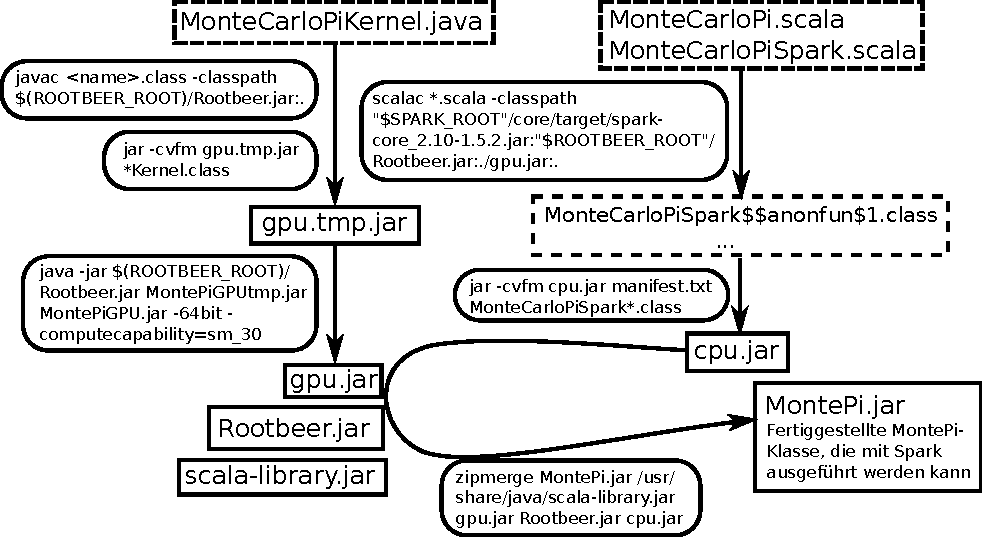
\includegraphics[width=1.15\linewidth]{compile-structure-deu-new-short.pdf}}
\end{frame}


\begin{frame}[fragile]
    \frametitle{Bemerkungen und Hinweise}
    %%%%NH: die folgenden Punkte finde ich gut, aber lieber am Schluss des Results-Kapitel einfügen. Kannst ja auch deine contributions+deren Effekt rootbeer erwähnen.
    %%%%NH: multi gpu fähigkeiten von rb erwähnen
    % sagen:
    %  - Leider wurde die meiste Bearbeitungszeit für diesen Beleg vom Lösen von Bugs beansprucht, sodass ich nicht darauf verzichten kann, zumindest einige davon zu erwähnen, auf dass sie jemanden helfen mögen, der einen ähnlichen Ansatz wie ich verfolgen möchte
    \begin{itemize}
        \item Nur Java 6 ist von Rootbeer offiziell unterstützt, Java 7 geht aber großteils, nicht aber Java 8
              %\begin{lstlisting}
              %    java.lang.NullPointerException
              %        at soot.rbclassload.RootbeerClassLoader.loadHierarchySootClasses(RootbeerClassLoader.java:963)
              %\end{lstlisting}
              % https://github.com/pcpratts/rootbeer1/issues/175 - Issues with jre1.8
        \item nur bis GCC 4.9 unterstützt % (wegen CUDA-Compiler)
        \item die Option \lstinline!-computecapability=sm_30! muss angegeben werden, da seit CUDA 7.0 die Standardarchitektur \lstinline!compute_12! nicht mehr unterstützt wird (korrekt nun \lstinline!sm_12!)
              %\begin{lstlisting}
              %    nvcc fatal   : Unsupported gpu architecture 'compute_12'
              %\end{lstlisting}
              % https://github.com/pcpratts/rootbeer1/issues/180 - CUDA 7.0: nvcc fatal: Unsupported gpu architecture 'compute_12'
        \item Automatische Kernel-Konfiguration hat einen Bug, der standardmäßig immer so viele Kernel startet wie gleichzeitig auf einem Shared Multiprozessor laufen können.
              % return new ThreadConfig( block_shaper.getMaxThreadsPerBlock(), 1, 1,
              %                          block_shaper.getMaxBlocksPerProc(), 1,
              % https://github.com/pcpratts/rootbeer1/issues/168
        \item Bug wo Rootbeer hat standardmäßig versucht den gesamten freien Speicher minus den benötigten zu alloziieren versuchte
              % sagen:
              %  - verhinderte multi-GPU, weil ein Kontext schon so gut wie den gesamten Speicher für sich beanspruchen wollte.
              %  - nur ein Problem mit multiple Rootbeer.jar
              % https://github.com/mxmlnkn/rootbeer1/commit/0d9699a40b06a7e5efee7213ca7fb215d6ef1377
              % https://github.com/mxmlnkn/rootbeer1/commit/cc2318673077a52f13a8c4b4d294fbd39e639ca5
              % /media/d/Studium/9TH SEMESTER/scaromare/MontePi/multiNode/multiGpu/scala$ /opt/spark-1.5.2/bin/spark-submit --master local[4] --class TestMonteCarloPi MontePi.jar 268435456 2
              %   16/01/22 03:27:59 ERROR Executor: Exception in task 1.0 in stage 0.0 (TID 1)
              %rg.trifort.rootbeer.runtime.CudaErrorException: CUDA_ERROR_OUT_OF_MEMORY: Error in cuMemAlloc: gpu_object_mem
              %   at org.trifort.rootbeer.runtime.CUDAContext.nativeBuildState(Native Method)
              %   at org.trifort.rootbeer.runtime.CUDAContext.access$1100(CUDAContext.java:17)
              %   at org.trifort.rootbeer.runtime.CUDAContext$GpuEventHandler.onEvent(CUDAContext.java:315)
              %   at org.trifort.rootbeer.runtime.CUDAContext$GpuEventHandler.onEvent(CUDAContext.java:308)
              %   at com.lmax.disruptor.BatchEventProcessor.run(BatchEventProcessor.java:128)
              %   at java.util.concurrent.ThreadPoolExecutor.runWorker(ThreadPoolExecutor.java:1145)
              %   at java.util.concurrent.ThreadPoolExecutor$Worker.run(ThreadPoolExecutor.java:615)
              %   at java.lang.Thread.run(Thread.java:745)
        \item die ausführbare jar für Spark darf kein Leerzeichen im Pfad enthalten:
              % $SPARK_ROOT/bin/spark-submit --master $MASTER_ADDRESS ./src/sort.py "$(pwd)"/data/The_Complete_Works_of_Willia.txt
              %   java.io.FileNotFoundException: Added file file:/media/f/Studium/9TH%20SEMESTER/scaromare/spark-gpu/src/sort.py does not exist.
              %      at org.apache.spark.SparkContext.addFile(SparkContext.scala:1365)
          %  - Alignement Bug in Speicherserialisierung
          %       https://github.com/mxmlnkn/rootbeer1/commit/cc2318673077a52f13a8c4b4d294fbd39e639ca5
        \item Zu kompilierende jar an Rootbeer >muss< auf .jar enden
              % normalerweise sollte die Dateiendung unter Linux egal sein, gibt Magic Bytes und Co
              % #Warning: the following soot-classpath entry is not a supported archive file (must be .zip, .jar or .apk): MontePiGPU.jar.tmp
        \item Profiling mit NVIDIA nvvp möglich. (Executable: java, Argumente: \lstinline!-jar ./MontePi.jar!)
      \end{itemize}
\end{frame}


%%%%%%%%%%%%%%%%%%%%%%%%%%%%%%%%%%%%%%%%%%%%%%%%%%%%%%%%%%%%%%%%%%%%%%%%%%%%%%%%
\section{Ergebnisse}
%%%%%%%%%%%%%%%%%%%%%%%%%%%%%%%%%%%%%%%%%%%%%%%%%%%%%%%%%%%%%%%%%%%%%%%%%%%%%%%%





%%%%NH: hardware auf der du deine tests durchgeführt hast beschreiben
%%%%NH: nochmal kurz den benchmark + motivation beschreiben  (use case => machine learning in labs). auch erwähnen, dass du eine cuda implementation erstellt hast ..
%%%%NH: spannend wäre, ob bottlenecks in der implementierung => allg. profiling von spark/rootbeer code // hast du bottlenecks entdeckt?

\begin{frame}[fragile]
    \frametitle{Leistungsanalyse: 1 CPU-Kern / GPU auf Taurus gpu2}
    \begin{lstlisting}[language=bash,breakautoindent=false,numbers=none]
salloc -p gpu2-interactive --nodes=1 --ntasks-per-node=1 --cpus-per-task=1 --gres=gpu:1 --time=02:00:00
\end{lstlisting}\vspace{-1.5\baselineskip}
    % Erstellt  mit:
    %   ssh taurus
    %   # Rootbeer commit ef79eaddc7956bf9bb3b9bd4d287e377e3949075
    %   ( git checkout a2302ec67b3f96df &&
    %     cd ~/scaromare/rootbeer1/csrc &&
    %     ./compile_linux_x64           &&
    %     cd ..                         &&
    %     ant jar                       &&
    %     ./pack-rootbeer )
    %   makeOpts=( \
    %       "SPARK_ROOT=$HOME/spark-1.5.2-bin-hadoop2.6" \
    %       "SPARKCORE_JAR=~/spark-1.5.2-bin-hadoop2.6/lib/spark-assembly-1.5.2-hadoop2.6.0.jar" \
    %       "SCALA_ROOT=$(dirname $(which scala))/../lib" \
    %   )
    %   cd ~/scaromare/MontePi
    %   git checkout
    %   make -B -C singleNode/singleCore/java/  "${makeOpts[@]}"  MontePi.jar
    %   make -B -C singleNode/singleCore/scala/ "${makeOpts[@]}"  MontePi.jar
    %   make -B -C singleNode/singleGpu/cpp/    "${makeOpts[@]}"  MontePi.jar
    %   make -B -C singleNode/multiGpu/java/    "${makeOpts[@]}"  MontePi.jar
    %   make -B -C singleNode/multiGpu/scala/   "${makeOpts[@]}"  MontePi.jar
    %   salloc -p gpu2-interactive --nodes=1 --ntasks-per-node=1 --cpus-per-task=1 --gres=gpu:1 --time=02:00:00
    %   ~/scaromare/MontePi/benchmarkImpl.sh
    %   cd scaromare/MontePi/
    %   python plot.py --workload-log 2016-07-02_01-18-12/results.log
    \centerline{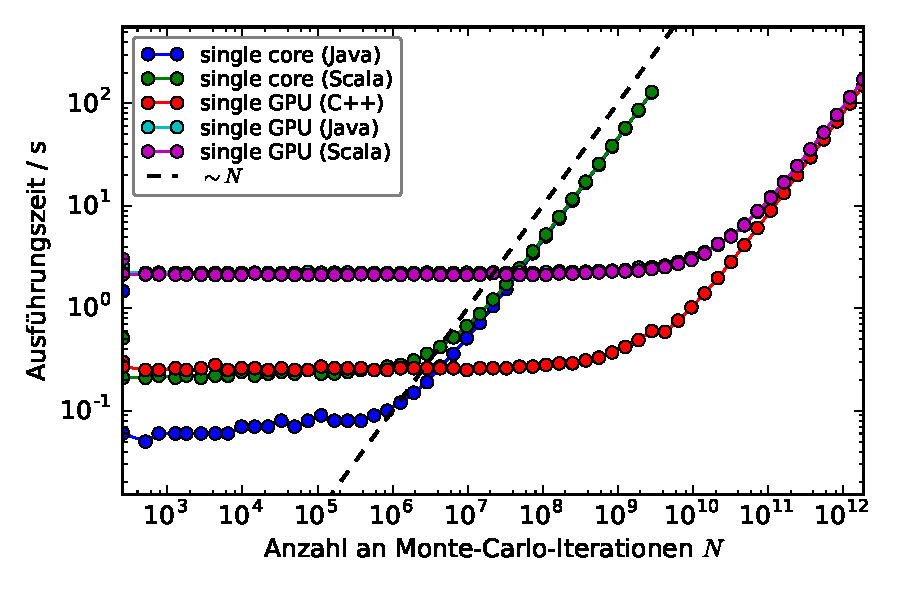
\includegraphics[width=0.9\linewidth]{benchmarks-workload-scaling.pdf}}
    % sagen:
    %   - benchmarkImpl.sh misst mittels 'time' Linuxshellbefehls
    %   - overhead ist riesig, für GPU vs CPU und für Java vs. C++ -> relativ große Probleme rentieren sich nur
    %   - Java wird für sehr große Probleme schneller als C++ -> Vorteil der automatischen Optimierungen durch die JVM durch Rootbeer! -> nächste Seite Profiler nur kurz erwähnen
\end{frame}

%%%%NH: multi gpu, multi node single gpu, multi node multi gpu, ...


\begin{frame}[fragile]
    \frametitle{Spark auf Taurus über Slurm starten}
    %\begin{itemize}
    %    \item Manuelle Installation von maven, ant, spark, zipmerge
    %    % für spark wurden precompiled binaries genommen, weil es bei der Kompilation auch Probleme gab, die nicht behoben werden konnten
    %\end{itemize}
    % This does similar things as vanilla $SPARK_ROOT/sbin/start-master.sh but slurm compatible, e.g. not in daemon-mode
    \begin{lstlisting}[language=bash]
function startSpark() {
  jobid=$(sbatch "$@" --output="$SPARK_LOGS/%j.out" --error="$SPARK_LOGS/%j.err" $HOME/scaromare/start_spark_slurm.sh)
  # wait for job to start
  export MASTER_ADDRESS=$(cat ~/spark/logs/${jobid}_spark_master)
}
\end{lstlisting}\vspace{-1.5\baselineskip}
\begin{lstlisting}[language=bash]
startSpark --time=04:00:00 --nodes=$((nodes+1)) --partition=gpu2 --gres=gpu:$gpusPerNode --cpus-per-task=$coresPerNode
~/spark-1.5.2-bin-hadoop2.6/bin/spark-submit --master $MASTER_ADDRESS ~/scaromare/MontePi/multiNode/multiGpu/scala/MontePi.jar $arguments
\end{lstlisting}
\end{frame}

\begin{frame}[fragile]
    \frametitle{\lstinline!start_spark_slurm.sh!}
    \begin{lstlisting}[language=bash,xleftmargin=0pt,linewidth=1.05\linewidth,basicstyle=\scriptsize]
if [ "$1" != 'sran' ]; then
  script=/scratch/$USER/${SLURM_JOBID}_$(basename "$0")
  cp "$0" "$script"
  export SPARK_DAEMON_MEMORY=$(( $SLURM_MEM_PER_CPU * $SLURM_CPUS_PER_TASK / 2 ))m
  export SPARK_WORKER_CORES=$SLURM_CPUS_PER_TASK
  srun "$script" 'sran' "$@"
else
  module load scala/2.10.4 java/jdk1.7.0_25 cuda/7.0.28
  if [ $SLURM_PROCID -eq 0 ]; then # if master start driver
    . "$SPARK_ROOT/sbin/spark-config.sh"
    . "$SPARK_ROOT/bin/load-spark-env.sh"
    "$SPARK_ROOT/bin/spark-class" org.apache.spark.deploy.master.Master --ip $(hostname) --port $SPARK_MASTER_PORT --webui-port $SPARK_MASTER_WEBUI_PORT
  else
    # convert "host20[39-40]" to "host2039"
    MASTER_NODE=spark://$(scontrol show hostname $SLURM_NODELIST | head -n 1):7077
    "$SPARK_ROOT/bin/spark-class" org.apache.spark.deploy.worker.Worker $MASTER_NODE
  fi
fi
\end{lstlisting}
% This section will be run when started by sbatch
%  export SPARK_ROOT=$HOME/spark-1.5.2-bin-hadoop2.6/
%  export SPARK_JAVA_OPTS+="-XX:+UseParallelGC -XX:MaxPermSize=5G"
%  export SPARK_MEM=$SPARK_DAEMON_MEMORY
%  export SPARK_WORKER_DIR=$HOME/spark/logs
%  export SPARK_LOCAL_DIRS=$(mktemp)
%  export SPARK_MASTER_PORT=7077
%  export SPARK_MASTER_WEBUI_PORT=8080
\end{frame}

\begin{frame}
    \frametitle{Benchmark Spark auf CPU}
    \centerline{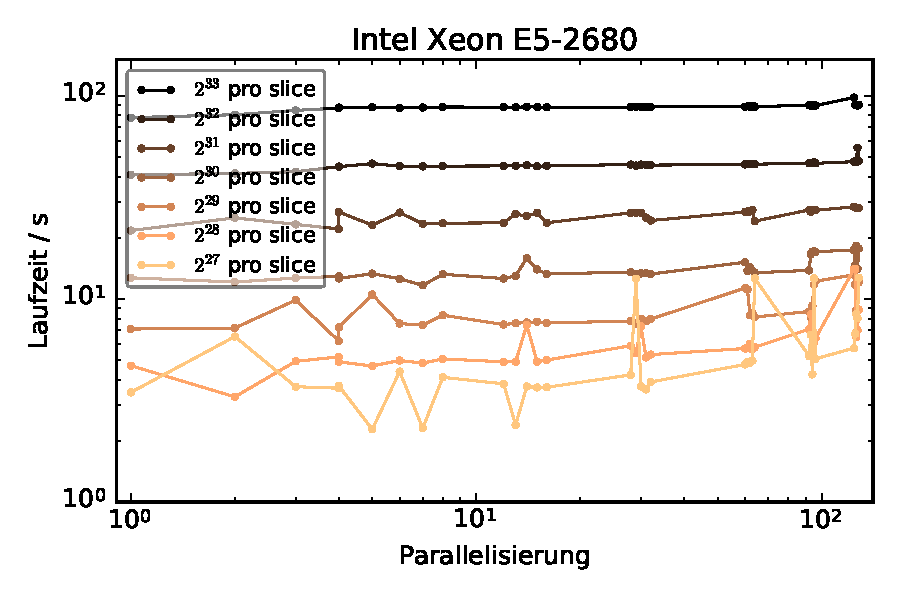
\includegraphics[width=0.9\linewidth]{cluster-strong-scaling-cpu.pdf}}
\end{frame}


\begin{frame}
    \frametitle{Benchmark Spark mit Rootbeer (alte Ergebnisse)}
    % "warum haben sie die neue Version nicht gebenchmarkt?" -> wegen Rootbeerproblemen -> deshalb rootbeer folie vor dieser
    \centerline{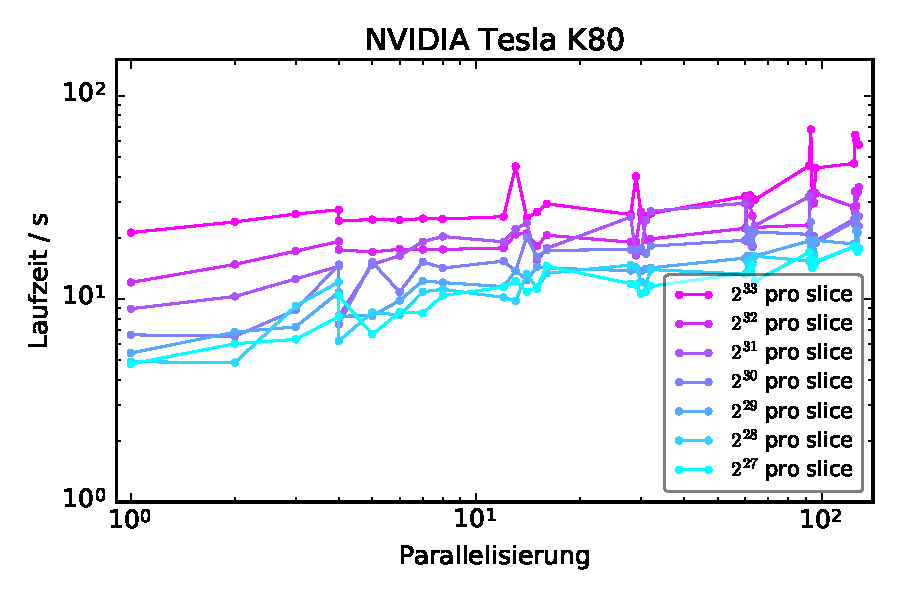
\includegraphics[width=0.9\linewidth]{cluster-strong-scaling-gpu.pdf}}
\end{frame}



%%%%%%%%%%%%%%%%%%%%%%%%%%%%%%%%%%%%%%%%%%%%%%%%%%%%%%%%%%%%%%%%%%%%%%%%%%%%%%%%
\section{Zusammenfassung}
%%%%%%%%%%%%%%%%%%%%%%%%%%%%%%%%%%%%%%%%%%%%%%%%%%%%%%%%%%%%%%%%%%%%%%%%%%%%%%%%
%%%%NH: Herr Nagel fragt gern: ``Was haben wir gelernt''
%%%%NH: => generell im Ausblick vielleicht noch erwähnen, was zukünftig (an deinem Framework, Rootbeer) verbessert werden sollte
%%%%NH: => z.B. gibt es möglichkeiten, um host-gpu transfers zu vermeiden/verringern
%%%%NH: verringerung der latenz durch einsatz neuer bustechnologien (nvlink)?
\begin{frame}
	\frametitle{Zusammenfassung}
	\begin{itemize}
		\item Kombination aus GPGPU mittels Rootbeer und Spark ausgetestet
            % -> das haben wir gelernt?
        \item Mehrere Bugfixes für Rootbeer geschrieben
            % -> und gelernt, dass man Ein-Mann-Projekte vlt.e her meiden sollte ... wenn man sie nicht eingenhändig weiterentwickeln will
        % \item Leider erfolglos
	\end{itemize}
    \textbf{Ausblick:}
    \begin{itemize}
        \item Codereview von Rootbeer oder andere GPU-API ist nötig
        %  java.lang.ClassCastException: MonteCarloPiKernel cannot be cast to [J
        %      at MonteCarloPiKernel.org_trifort_readFromHeapRefFields_MonteCarloPiKernel0(Jasmin)
        %      at MonteCarloPiKernelSerializer.doReadFromHeap(Jasmin)
        %      at org.trifort.rootbeer.runtime.Serializer.readFromHeap(Serializer.java:155)
        %      at org.trifort.rootbeer.runtime.CUDAContext.readBlocksList(CUDAContext.java:452)
        %      at org.trifort.rootbeer.runtime.CUDAContext$GpuEventHandler.onEvent(CUDAContext.java:332)
        %      at org.trifort.rootbeer.runtime.CUDAContext$GpuEventHandler.onEvent(CUDAContext.java:308)
        %      at com.lmax.disruptor.BatchEventProcessor.run(BatchEventProcessor.java:128)
        %      at java.util.concurrent.ThreadPoolExecutor.runWorker(ThreadPoolExecutor.java:1145)
        %      at java.util.concurrent.ThreadPoolExecutor$Worker.run(ThreadPoolExecutor.java:615)
        %      at java.lang.Thread.run(Thread.java:724)
        %
        % java.lang.NullPointerException
        %     at org.trifort.rootbeer.runtime.Serializer.checkWriteCache(Serializer.java:91)
        %     at org.trifort.rootbeer.runtime.Serializer.writeToHeap(Serializer.java:117)
        %     at MonteCarloPiKernel.org_trifort_writeToHeapRefFields_MonteCarloPiKernel0(Jasmin)
        %     at MonteCarloPiKernelSerializer.doWriteToHeap(Jasmin)
        %     at org.trifort.rootbeer.runtime.Serializer.writeToHeap(Serializer.java:127)
        %     at org.trifort.rootbeer.runtime.Serializer.writeToHeap(Serializer.java:44)
        %     at org.trifort.rootbeer.runtime.CUDAContext.writeBlocksList(CUDAContext.java:500)
        %     at org.trifort.rootbeer.runtime.CUDAContext.access$1400(CUDAContext.java:24)
        %     at org.trifort.rootbeer.runtime.CUDAContext$GpuEventHandler.onEvent(CUDAContext.java:419)
        %     at org.trifort.rootbeer.runtime.CUDAContext$GpuEventHandler.onEvent(CUDAContext.java:373)
        %     at com.lmax.disruptor.BatchEventProcessor.run(BatchEventProcessor.java:128)
        %     at java.util.concurrent.ThreadPoolExecutor.runWorker(ThreadPoolExecutor.java:1145)
        %     at java.util.concurrent.ThreadPoolExecutor$Worker.run(ThreadPoolExecutor.java:615)
        %     at java.lang.Thread.run(Thread.java:724)

       \item heterogene Berechnungen auf CPU + GPU % sagen: sollten sehr einfach möglich sein, da Rootbeer asynchron unterstützt (although I don't think there is somehting like: peek yet), und da gpuMethod von Host aufrufbar ist ( wäre riesen Vorteil von Rootbeer, dass der Spark-Nutzer kein CUDA oder ähnliches schreiben muss ... durch den Vorteil fallen Alternativen mehr oder minder alle raus )  ( so heterogen kann aber nur einen CPU core pro GPU nutzen.. häufig aber mehr cores als CPUs :S... wäre also doch bisschen mehr dahinter. Außerdem kann man glaube nicht mehr spark partitionen auf einen Knoten starten, als er CPU cores hat, d.h. einige Partitionen müssten CPU+GPU starten, während andere nur CPU starten.. Weiteres Problem ist, dass man nicht weiß, wie lange das jeweils dauert. Wenn man CPU+GPU vom selben Programm startet, dann kann man sehr kleine Arbeitslasten an die CPU senden und dann immer in einer Schleife schauen, ob die GPU schon fertig ist. Aber die Partitionen, die nur CPU haben werden immer eher oder später fertig sein. ... wird möglicherweise doch schwieriger als gedacht ...)
       \item Erweiterung von Rootbeer um neue Features wie NVIDIA NVLink
       \item Implementation direkt in Spark würde z.B. cache/persist auf GPUs erlauben, um Host-GPU-Transfers zu sparen
                % glaube cache/persist erkläre ich bei Spark irgendwann oben.
    \end{itemize}
\end{frame}


\end{document}

